\section{Introduction}
\label{sec:introduction}

An experiment can finish without reproducing the claim it appears to test.  A run may emit a checkpoint and a metric even when the source protocol does not uniquely determine the target, split, preprocessing, or hyperparameters.  Conversely, a faithfully specified method may fail for an ordinary engineering reason and never yield a comparable number.  Treating these outcomes as one binary label---``reproduced'' or ``not reproduced''---hides the evidence needed to interpret a forecasting benchmark.

This distinction is consequential in urban electric-vehicle (EV) charging forecasting.  Open resources now cover zonal charging demand in Shenzhen, station occupancy in Paris, workplace charging sessions, and harmonized measurements across cities and continents \cite{li2025urbanev,amaraouali2024smarter,amaraouali2023parisdataset,lee2019acndata,guo2025charged}.  These resources do not define interchangeable prediction problems: occupancy rates, port states, session records, charging duration, and energy volume have different denominators, missingness mechanisms, and operational meanings.  At the same time, the associated modeling literature spans physics-informed graph networks, language-model formulations, exogenous-variable Transformers, linear decompositions, and pretrained forecasters \cite{qu2024pag,qu2024chatev,wang2024timexer,zeng2023dlinear,ansari2024chronos,ansari2025chronos2}.  A reported score therefore becomes interpretable only after the data semantics, information set, forecast origin, and evaluation protocol are fixed.

Forecasting research has long emphasized out-of-sample and rolling-origin evaluation \cite{dawid1984prequential,tashman2000oos}.  More recent guidance documents leakage through preprocessing, inappropriate random splits, weak benchmarks, and metric choices that do not match the data or decision problem \cite{hewamalage2023pitfalls,kapoor2023leakage}.  Reproducibility programs likewise encourage code, data, environment, and reporting artifacts \cite{pineau2021reproducibility}.  These practices are necessary, but a remaining gap is operational: once a large matrix has been partially recovered and executed, how should a researcher distinguish disclosure quality from execution status, predictive opportunity from realizable gain, and a statistically detectable difference from an improvement large enough to justify added serving cost?  Without explicit distinctions, additional model search can gradually convert an evaluation interval into a tuning resource.

We address this gap through an artifact-grounded case audit of one UrbanEV forecasting inventory and its subsequent model-development chain.  The intended readers are benchmark authors, artifact evaluators, and reviewers who must decide which urban-forecasting claims are licensed by a heterogeneous experiment record.  The audit freezes a six-state configuration taxonomy, verifies target and run identities, and follows each proposed improvement through a sequential evidence ladder.  That ladder separates an infeasible oracle diagnostic, forecast-origin predictability, strict prequential fixed fusion, learned routing, synchronous latency, foundation-model teacher qualification, residual distillation, and development-only replication on a separately isolated Paris panel.  Fail-closed metric locks prevent incomplete or invalid artifacts from entering aggregate results, while internally time-stamped minimum-effect gates determine whether a stage authorizes the next one.  The contribution is an auditable claim grammar and workflow instantiated by this case, not evidence that the framework has already reduced false discoveries across independent teams.

The audit changes the apparent story.  Of 1,224 frozen configurations, 865 have completed artifacts, but only 156 satisfy the joint exact-protocol-and-numerical criterion.  In the internal UrbanEV rolling evaluation, a strictly fitted CAPER--TimeXer fusion reduces macro RMSE by 3.178\% relative to the strongest evaluated single model, yet increases batch-1 median synchronous latency by 48.86\% on the frozen laptop-GPU workload.  A learned router adds only 0.443\% over that fixed reference and therefore fails the internally time-stamped 1\% progression gate despite a positive block-bootstrap interval.  The same discipline rejects Chronos-2 as the project teacher under the exact UrbanEV protocol, stops residual distillation after a 0.119\% gain over ground-truth-only training, and withholds student training on Paris when a strict development-only teacher improves by 0.847\% rather than the required 1\%.  These are scoped gate outcomes, not general verdicts about routing, foundation models, or distillation.

We organize the study around four research questions:

\begin{enumerate}
    \item[\textbf{RQ1}] How much of a large forecasting configuration matrix is exactly reproducible, approximately recoverable, trend-only, underidentified, failed, or never completed?
    \item[\textbf{RQ2}] When two experts are complementary, how much of an infeasible oracle gap survives strict prequential fixed fusion and learned routing?
    \item[\textbf{RQ3}] How do apparent accuracy gains change once synchronous inference latency and a frozen minimum-effect threshold are enforced?
    \item[\textbf{RQ4}] How do fail-closed audits, control branches, independent evidence, and stopping rules change the claims that remain defensible?
\end{enumerate}

This paper makes four contributions:

\begin{itemize}
    \item \textbf{A configuration-level evidence taxonomy.}  We separate protocol and numerical reproduction, disclosure-limited recovery, trend-only recovery, underidentification, execution failure, and non-completion for a frozen 1,224-configuration inventory.  The resulting registry makes clear why execution completion is not a substitute for exact reproduction.
    \item \textbf{A portable audit framework and claim grammar.}  We type evidence objects as configuration, prediction, target, metric, latency, or protected-storage artifacts; attach identity and lock requirements; and specify the narrow wording each evidence state authorizes.  A claim-to-artifact ledger and reviewer checklist make the framework inspectable rather than leaving it as project history.
    \item \textbf{A sequential audit of model-improvement claims.}  We connect target-identity checks, prequential fitting, control branches, block-resampled uncertainty, and hardware-specific latency to explicit authorization gates.  This exposes where theoretical complementarity becomes a material fixed-fusion gain and where later routing, teacher, and distillation signals remain below their frozen effect requirements.
    \item \textbf{A fail-closed evidence boundary.}  We document audit events that blocked invalid shuffled controls and repaired missing-target representation before metric access, and we procedurally isolate Paris formal and protected target-bearing sources so that only development targets contribute analytically.  The workflow produces an auditable mapping from each numerical statement to its protocol, artifact, and permitted wording.
\end{itemize}

\begin{figure}[htbp]
    \centering
    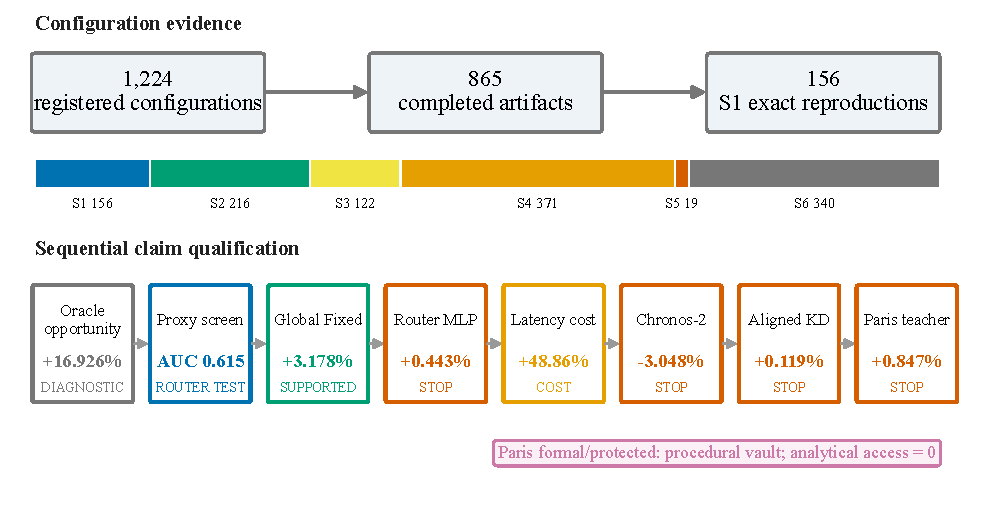
\includegraphics[width=0.9\linewidth]{figures/fig01_evidence_ladder.pdf}
    \caption{The audit separates registration, completed execution, exact reproduction, predictive opportunity, measured engineering cost, and qualification.  A positive diagnostic or comparison does not automatically authorize the next stage; Paris formal and protected targets remain in procedural vault-only storage with zero analytical use.}
    \label{fig:evidence-ladder}
\end{figure}

\paragraph{Claim boundary.}
This is an empirical audit and evaluation study, not a new state-of-the-art model paper.  Its numerical conclusions concern one UrbanEV inventory, six internal rolling folds at seed 42, one frozen latency platform, and Paris development-only evidence.  UrbanEV and Paris absolute RMSE values are not compared because the panels and targets differ.  The 1\% threshold is an internally time-stamped project convention, not a universal definition of scientific or economic significance.  Neither Paris formal nor Paris protected targets are accessed analytically, and we make no claim of protected-test performance, production readiness, universal generalization, or cross-dataset superiority.  Their movement into independent vault-only storage is recorded as a storage event rather than concealed as non-materialization.  Within that boundary, the case shows how configuration identifiability and sequential evidence controls constrain the claims this forecasting program can support.

The remainder of the paper first relates this audit to EV forecasting resources, time-series evaluation, and reproducibility research.  It then defines the evidence taxonomy and sequential protocol, reports the registry and model-chain results, analyzes the fail-closed events and claim boundaries, and concludes with implications for auditable forecasting studies.
